\documentclass[1p]{elsarticle_modified}
%\bibliographystyle{elsarticle-num}

%\usepackage[colorlinks]{hyperref}
%\usepackage{abbrmath_seonhwa} %\Abb, \Ascr, \Acal ,\Abf, \Afrak
\usepackage{amsfonts}
\usepackage{amssymb}
\usepackage{amsmath}
\usepackage{amsthm}
\usepackage{scalefnt}
\usepackage{amsbsy}
\usepackage{kotex}
\usepackage{caption}
\usepackage{subfig}
\usepackage{color}
\usepackage{graphicx}
\usepackage{xcolor} %% white, black, red, green, blue, cyan, magenta, yellow
\usepackage{float}
\usepackage{setspace}
\usepackage{hyperref}

\usepackage{tikz}
\usetikzlibrary{arrows}

\usepackage{multirow}
\usepackage{array} % fixed length table
\usepackage{hhline}

%%%%%%%%%%%%%%%%%%%%%
\makeatletter
\renewcommand*\env@matrix[1][\arraystretch]{%
	\edef\arraystretch{#1}%
	\hskip -\arraycolsep
	\let\@ifnextchar\new@ifnextchar
	\array{*\c@MaxMatrixCols c}}
\makeatother %https://tex.stackexchange.com/questions/14071/how-can-i-increase-the-line-spacing-in-a-matrix
%%%%%%%%%%%%%%%

\usepackage[normalem]{ulem}

\newcommand{\msout}[1]{\ifmmode\text{\sout{\ensuremath{#1}}}\else\sout{#1}\fi}
%SOURCE: \msout is \stkout macro in https://tex.stackexchange.com/questions/20609/strikeout-in-math-mode

\newcommand{\cancel}[1]{
	\ifmmode
	{\color{red}\msout{#1}}
	\else
	{\color{red}\sout{#1}}
	\fi
}

\newcommand{\add}[1]{
	{\color{blue}\uwave{#1}}
}

\newcommand{\replace}[2]{
	\ifmmode
	{\color{red}\msout{#1}}{\color{blue}\uwave{#2}}
	\else
	{\color{red}\sout{#1}}{\color{blue}\uwave{#2}}
	\fi
}

\newcommand{\Sol}{\mathcal{S}} %segment
\newcommand{\D}{D} %diagram
\newcommand{\A}{\mathcal{A}} %arc


%%%%%%%%%%%%%%%%%%%%%%%%%%%%%5 test

\def\sl{\operatorname{\textup{SL}}(2,\Cbb)}
\def\psl{\operatorname{\textup{PSL}}(2,\Cbb)}
\def\quan{\mkern 1mu \triangleright \mkern 1mu}

\theoremstyle{definition}
\newtheorem{thm}{Theorem}[section]
\newtheorem{prop}[thm]{Proposition}
\newtheorem{lem}[thm]{Lemma}
\newtheorem{ques}[thm]{Question}
\newtheorem{cor}[thm]{Corollary}
\newtheorem{defn}[thm]{Definition}
\newtheorem{exam}[thm]{Example}
\newtheorem{rmk}[thm]{Remark}
\newtheorem{alg}[thm]{Algorithm}

\newcommand{\I}{\sqrt{-1}}
\begin{document}

%\begin{frontmatter}
%
%\title{Boundary parabolic representations of knots up to 8 crossings}
%
%%% Group authors per affiliation:
%\author{Yunhi Cho} 
%\address{Department of Mathematics, University of Seoul, Seoul, Korea}
%\ead{yhcho@uos.ac.kr}
%
%
%\author{Seonhwa Kim} %\fnref{s_kim}}
%\address{Center for Geometry and Physics, Institute for Basic Science, Pohang, 37673, Korea}
%\ead{ryeona17@ibs.re.kr}
%
%\author{Hyuk Kim}
%\address{Department of Mathematical Sciences, Seoul National University, Seoul 08826, Korea}
%\ead{hyukkim@snu.ac.kr}
%
%\author{Seokbeom Yoon}
%\address{Department of Mathematical Sciences, Seoul National University, Seoul, 08826,  Korea}
%\ead{sbyoon15@snu.ac.kr}
%
%\begin{abstract}
%We find all boundary parabolic representation of knots up to 8 crossings.
%
%\end{abstract}
%\begin{keyword}
%    \MSC[2010] 57M25 
%\end{keyword}
%
%\end{frontmatter}

%\linenumbers
%\tableofcontents
%
\newcommand\colored[1]{\textcolor{white}{\rule[-0.35ex]{0.8em}{1.4ex}}\kern-0.8em\color{red} #1}%
%\newcommand\colored[1]{\textcolor{white}{ #1}\kern-2.17ex	\textcolor{white}{ #1}\kern-1.81ex	\textcolor{white}{ #1}\kern-2.15ex\color{red}#1	}

{\Large $\underline{12a_{0566}~(K12a_{0566})}$}

\setlength{\tabcolsep}{10pt}
\renewcommand{\arraystretch}{1.6}
\vspace{1cm}\begin{tabular}{m{100pt}>{\centering\arraybackslash}m{274pt}}
\multirow{5}{120pt}{
	\centering
	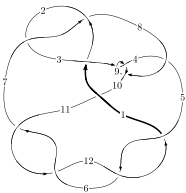
\includegraphics[width=112pt]{../../../GIT/diagram.site/Diagrams/png/1367_12a_0566.png}\\
\ \ \ A knot diagram\footnotemark}&
\allowdisplaybreaks
\textbf{Linearized knot diagam} \\
\cline{2-2}
 &
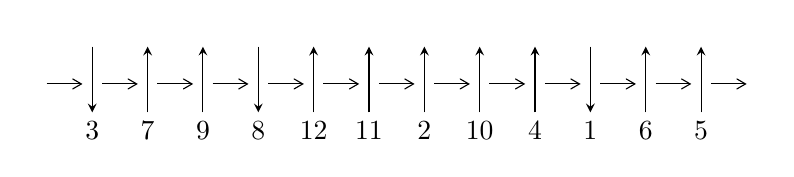
\begin{tikzpicture}[x=20pt, y=17pt]
	% nodes
	\node (C0) at (0, 0) {};
	\node (C1) at (1, 0) {};
	\node (C1U) at (1, +1) {};
	\node (C1D) at (1, -1) {3};

	\node (C2) at (2, 0) {};
	\node (C2U) at (2, +1) {};
	\node (C2D) at (2, -1) {7};

	\node (C3) at (3, 0) {};
	\node (C3U) at (3, +1) {};
	\node (C3D) at (3, -1) {9};

	\node (C4) at (4, 0) {};
	\node (C4U) at (4, +1) {};
	\node (C4D) at (4, -1) {8};

	\node (C5) at (5, 0) {};
	\node (C5U) at (5, +1) {};
	\node (C5D) at (5, -1) {12};

	\node (C6) at (6, 0) {};
	\node (C6U) at (6, +1) {};
	\node (C6D) at (6, -1) {11};

	\node (C7) at (7, 0) {};
	\node (C7U) at (7, +1) {};
	\node (C7D) at (7, -1) {2};

	\node (C8) at (8, 0) {};
	\node (C8U) at (8, +1) {};
	\node (C8D) at (8, -1) {10};

	\node (C9) at (9, 0) {};
	\node (C9U) at (9, +1) {};
	\node (C9D) at (9, -1) {4};

	\node (C10) at (10, 0) {};
	\node (C10U) at (10, +1) {};
	\node (C10D) at (10, -1) {1};

	\node (C11) at (11, 0) {};
	\node (C11U) at (11, +1) {};
	\node (C11D) at (11, -1) {6};

	\node (C12) at (12, 0) {};
	\node (C12U) at (12, +1) {};
	\node (C12D) at (12, -1) {5};
	\node (C13) at (13, 0) {};

	% arrows
	\draw[->,>={angle 60}]
	(C0) edge (C1) (C1) edge (C2) (C2) edge (C3) (C3) edge (C4) (C4) edge (C5) (C5) edge (C6) (C6) edge (C7) (C7) edge (C8) (C8) edge (C9) (C9) edge (C10) (C10) edge (C11) (C11) edge (C12) (C12) edge (C13) ;	\draw[->,>=stealth]
	(C1U) edge (C1D) (C2D) edge (C2U) (C3D) edge (C3U) (C4U) edge (C4D) (C5D) edge (C5U) (C6D) edge (C6U) (C7D) edge (C7U) (C8D) edge (C8U) (C9D) edge (C9U) (C10U) edge (C10D) (C11D) edge (C11U) (C12D) edge (C12U) ;
	\end{tikzpicture} \\
\hhline{~~} \\& 
\textbf{Solving Sequence} \\ \cline{2-2} 
 &
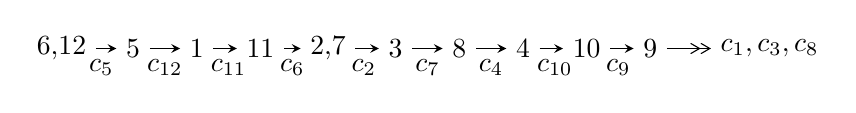
\begin{tikzpicture}[x=23pt, y=7pt]
	% node
	\node (A0) at (-1/8, 0) {6,12};
	\node (A1) at (1, 0) {5};
	\node (A2) at (2, 0) {1};
	\node (A3) at (3, 0) {11};
	\node (A4) at (65/16, 0) {2,7};
	\node (A5) at (41/8, 0) {3};
	\node (A6) at (49/8, 0) {8};
	\node (A7) at (57/8, 0) {4};
	\node (A8) at (65/8, 0) {10};
	\node (A9) at (73/8, 0) {9};
	\node (C1) at (1/2, -1) {$c_{5}$};
	\node (C2) at (3/2, -1) {$c_{12}$};
	\node (C3) at (5/2, -1) {$c_{11}$};
	\node (C4) at (7/2, -1) {$c_{6}$};
	\node (C5) at (37/8, -1) {$c_{2}$};
	\node (C6) at (45/8, -1) {$c_{7}$};
	\node (C7) at (53/8, -1) {$c_{4}$};
	\node (C8) at (61/8, -1) {$c_{10}$};
	\node (C9) at (69/8, -1) {$c_{9}$};
	\node (A10) at (11, 0) {$c_{1},c_{3},c_{8}$};

	% edge
	\draw[->,>=stealth]	
	(A0) edge (A1) (A1) edge (A2) (A2) edge (A3) (A3) edge (A4) (A4) edge (A5) (A5) edge (A6) (A6) edge (A7) (A7) edge (A8) (A8) edge (A9) ;
	\draw[->>,>={angle 60}]	
	(A9) edge (A10);
\end{tikzpicture} \\ 

\end{tabular} \\

\footnotetext{
The image of knot diagram is generated by the software ``\textbf{Draw programme}" developed by Andrew Bartholomew(\url{http://www.layer8.co.uk/maths/draw/index.htm\#Running-draw}), where we modified some parts for our purpose(\url{https://github.com/CATsTAILs/LinksPainter}).
}\phantom \\ \newline 
\centering \textbf{Ideals for irreducible components\footnotemark of $X_{\text{par}}$} 
 
\begin{align*}
I^u_{1}&=\langle 
1.48359\times10^{42} u^{84}+1.49960\times10^{42} u^{83}+\cdots+3.29594\times10^{42} b-1.20784\times10^{43},\\
\phantom{I^u_{1}}&\phantom{= \langle  }2.21165\times10^{41} u^{84}+2.55434\times10^{41} u^{83}+\cdots+8.23985\times10^{41} a+1.14680\times10^{42},\;u^{85}+u^{84}+\cdots+5 u+1\rangle \\
I^u_{2}&=\langle 
- u^2 a+u^3+b- a+3 u,\;-2 u^3 a+u^3+a^2-8 a u- a+4 u-4,\;u^4+3 u^2+1\rangle \\
\\
\end{align*}
\raggedright * 2 irreducible components of $\dim_{\mathbb{C}}=0$, with total 93 representations.\\
\footnotetext{All coefficients of polynomials are rational numbers. But the coefficients are sometimes approximated in decimal forms when there is not enough margin.}
\newpage
\renewcommand{\arraystretch}{1}
\centering \section*{I. $I^u_{1}= \langle 1.48\times10^{42} u^{84}+1.50\times10^{42} u^{83}+\cdots+3.30\times10^{42} b-1.21\times10^{43},\;2.21\times10^{41} u^{84}+2.55\times10^{41} u^{83}+\cdots+8.24\times10^{41} a+1.15\times10^{42},\;u^{85}+u^{84}+\cdots+5 u+1 \rangle$}
\flushleft \textbf{(i) Arc colorings}\\
\begin{tabular}{m{7pt} m{180pt} m{7pt} m{180pt} }
\flushright $a_{6}=$&$\begin{pmatrix}1\\0\end{pmatrix}$ \\
\flushright $a_{12}=$&$\begin{pmatrix}0\\u\end{pmatrix}$ \\
\flushright $a_{5}=$&$\begin{pmatrix}1\\u^2\end{pmatrix}$ \\
\flushright $a_{1}=$&$\begin{pmatrix}u\\u^3+u\end{pmatrix}$ \\
\flushright $a_{11}=$&$\begin{pmatrix}- u\\u\end{pmatrix}$ \\
\flushright $a_{2}=$&$\begin{pmatrix}-0.268409 u^{84}-0.309998 u^{83}+\cdots-2.53477 u-1.39178\\-0.450127 u^{84}-0.454986 u^{83}+\cdots+16.2601 u+3.66462\end{pmatrix}$ \\
\flushright $a_{7}=$&$\begin{pmatrix}u^2+1\\- u^2\end{pmatrix}$ \\
\flushright $a_{3}=$&$\begin{pmatrix}0.706834 u^{84}+0.799119 u^{83}+\cdots+14.4948 u+2.69792\\0.649070 u^{84}+0.131711 u^{83}+\cdots+16.4414 u+3.28599\end{pmatrix}$ \\
\flushright $a_{8}=$&$\begin{pmatrix}-4.29653 u^{84}-2.10680 u^{83}+\cdots-24.9777 u+0.363311\\0.945075 u^{84}-0.221620 u^{83}+\cdots+0.773811 u+0.688980\end{pmatrix}$ \\
\flushright $a_{4}=$&$\begin{pmatrix}3.13890 u^{84}+2.19012 u^{83}+\cdots+23.1159 u+1.31435\\1.00849 u^{84}-0.279889 u^{83}+\cdots-14.1954 u-4.54399\end{pmatrix}$ \\
\flushright $a_{10}=$&$\begin{pmatrix}u^5+2 u^3- u\\u^7+3 u^5+2 u^3+u\end{pmatrix}$ \\
\flushright $a_{9}=$&$\begin{pmatrix}-2.98788 u^{84}-2.09995 u^{83}+\cdots-26.9778 u-1.05953\\-0.483470 u^{84}-0.327238 u^{83}+\cdots+1.60308 u+1.52630\end{pmatrix}$\\&\end{tabular}
\flushleft \textbf{(ii) Obstruction class $= -1$}\\~\\
\flushleft \textbf{(iii) Cusp Shapes $= 3.44824 u^{84}+3.41811 u^{83}+\cdots+56.6384 u+20.3411$}\\~\\
\newpage\renewcommand{\arraystretch}{1}
\flushleft \textbf{(iv) u-Polynomials at the component}\newline \\
\begin{tabular}{m{50pt}|m{274pt}}
Crossings & \hspace{64pt}u-Polynomials at each crossing \\
\hline $$\begin{aligned}c_{1}\end{aligned}$$&$\begin{aligned}
&u^{85}+43 u^{84}+\cdots+72 u-16
\end{aligned}$\\
\hline $$\begin{aligned}c_{2},c_{7}\end{aligned}$$&$\begin{aligned}
&u^{85}+u^{84}+\cdots-12 u-4
\end{aligned}$\\
\hline $$\begin{aligned}c_{3},c_{9}\end{aligned}$$&$\begin{aligned}
&u^{85}+u^{84}+\cdots- u-5
\end{aligned}$\\
\hline $$\begin{aligned}c_{4}\end{aligned}$$&$\begin{aligned}
&u^{85}+3 u^{84}+\cdots-6487 u-28835
\end{aligned}$\\
\hline $$\begin{aligned}c_{5},c_{6},c_{11}\\c_{12}\end{aligned}$$&$\begin{aligned}
&u^{85}- u^{84}+\cdots+5 u-1
\end{aligned}$\\
\hline $$\begin{aligned}c_{8}\end{aligned}$$&$\begin{aligned}
&u^{85}-41 u^{84}+\cdots+131 u-25
\end{aligned}$\\
\hline $$\begin{aligned}c_{10}\end{aligned}$$&$\begin{aligned}
&u^{85}-23 u^{84}+\cdots+41 u-283
\end{aligned}$\\
\hline
\end{tabular}\\~\\
\newpage\renewcommand{\arraystretch}{1}
\flushleft \textbf{(v) Riley Polynomials at the component}\newline \\
\begin{tabular}{m{50pt}|m{274pt}}
Crossings & \hspace{64pt}Riley Polynomials at each crossing \\
\hline $$\begin{aligned}c_{1}\end{aligned}$$&$\begin{aligned}
&y^{85}+7 y^{84}+\cdots+31264 y-256
\end{aligned}$\\
\hline $$\begin{aligned}c_{2},c_{7}\end{aligned}$$&$\begin{aligned}
&y^{85}+43 y^{84}+\cdots+72 y-16
\end{aligned}$\\
\hline $$\begin{aligned}c_{3},c_{9}\end{aligned}$$&$\begin{aligned}
&y^{85}-41 y^{84}+\cdots+131 y-25
\end{aligned}$\\
\hline $$\begin{aligned}c_{4}\end{aligned}$$&$\begin{aligned}
&y^{85}+19 y^{84}+\cdots-11204895241 y-831457225
\end{aligned}$\\
\hline $$\begin{aligned}c_{5},c_{6},c_{11}\\c_{12}\end{aligned}$$&$\begin{aligned}
&y^{85}+99 y^{84}+\cdots-9 y-1
\end{aligned}$\\
\hline $$\begin{aligned}c_{8}\end{aligned}$$&$\begin{aligned}
&y^{85}+11 y^{84}+\cdots-6589 y-625
\end{aligned}$\\
\hline $$\begin{aligned}c_{10}\end{aligned}$$&$\begin{aligned}
&y^{85}-9 y^{84}+\cdots+1664023 y-80089
\end{aligned}$\\
\hline
\end{tabular}\\~\\
\newpage\flushleft \textbf{(vi) Complex Volumes and Cusp Shapes}
$$\begin{array}{c|c|c}  
\text{Solutions to }I^u_{1}& \I (\text{vol} + \sqrt{-1}CS) & \text{Cusp shape}\\
 \hline 
\begin{aligned}
u &= -0.269016 + 0.961532 I \\
a &= \phantom{-}1.34501 + 0.86076 I \\
b &= -0.677659 + 0.501079 I\end{aligned}
 & -1.44363 + 5.72996 I & \phantom{-0.000000 } 0 \\ \hline\begin{aligned}
u &= -0.269016 - 0.961532 I \\
a &= \phantom{-}1.34501 - 0.86076 I \\
b &= -0.677659 - 0.501079 I\end{aligned}
 & -1.44363 - 5.72996 I & \phantom{-0.000000 } 0 \\ \hline\begin{aligned}
u &= -0.015593 + 0.966863 I \\
a &= \phantom{-}0.574880 + 0.741720 I \\
b &= -0.201759 + 0.491321 I\end{aligned}
 & -0.320817 - 1.348260 I & \phantom{-0.000000 } 0 \\ \hline\begin{aligned}
u &= -0.015593 - 0.966863 I \\
a &= \phantom{-}0.574880 - 0.741720 I \\
b &= -0.201759 - 0.491321 I\end{aligned}
 & -0.320817 + 1.348260 I & \phantom{-0.000000 } 0 \\ \hline\begin{aligned}
u &= -0.547823 + 0.722739 I \\
a &= -1.92103 - 1.40701 I \\
b &= \phantom{-}0.484593 - 0.384674 I\end{aligned}
 & \phantom{-}0.66837 - 12.95260 I & \phantom{-0.000000 } 0 \\ \hline\begin{aligned}
u &= -0.547823 - 0.722739 I \\
a &= -1.92103 + 1.40701 I \\
b &= \phantom{-}0.484593 + 0.384674 I\end{aligned}
 & \phantom{-}0.66837 + 12.95260 I & \phantom{-0.000000 } 0 \\ \hline\begin{aligned}
u &= \phantom{-}0.244367 + 0.865284 I \\
a &= -1.22863 + 1.21755 I \\
b &= \phantom{-}0.628112 + 0.266767 I\end{aligned}
 & -3.62434 - 1.21550 I & \phantom{-0.000000 } 0 \\ \hline\begin{aligned}
u &= \phantom{-}0.244367 - 0.865284 I \\
a &= -1.22863 - 1.21755 I \\
b &= \phantom{-}0.628112 - 0.266767 I\end{aligned}
 & -3.62434 + 1.21550 I & \phantom{-0.000000 } 0 \\ \hline\begin{aligned}
u &= \phantom{-}0.519121 + 0.704971 I \\
a &= \phantom{-}1.90749 - 1.30014 I \\
b &= -0.328379 - 0.431956 I\end{aligned}
 & -1.71613 + 7.78904 I & \phantom{-0.000000 } 0 \\ \hline\begin{aligned}
u &= \phantom{-}0.519121 - 0.704971 I \\
a &= \phantom{-}1.90749 + 1.30014 I \\
b &= -0.328379 + 0.431956 I\end{aligned}
 & -1.71613 - 7.78904 I & \phantom{-0.000000 } 0\\
 \hline 
 \end{array}$$\newpage$$\begin{array}{c|c|c}  
\text{Solutions to }I^u_{1}& \I (\text{vol} + \sqrt{-1}CS) & \text{Cusp shape}\\
 \hline 
\begin{aligned}
u &= \phantom{-}0.539376 + 0.649975 I \\
a &= \phantom{-}0.680041 + 0.389729 I \\
b &= -0.387247 + 0.236701 I\end{aligned}
 & \phantom{-}3.03875 + 7.48933 I & \phantom{-0.000000 } 0 \\ \hline\begin{aligned}
u &= \phantom{-}0.539376 - 0.649975 I \\
a &= \phantom{-}0.680041 - 0.389729 I \\
b &= -0.387247 - 0.236701 I\end{aligned}
 & \phantom{-}3.03875 - 7.48933 I & \phantom{-0.000000 } 0 \\ \hline\begin{aligned}
u &= -0.546508 + 0.643529 I \\
a &= -1.67110 - 1.27874 I \\
b &= \phantom{-}0.206900 - 0.158340 I\end{aligned}
 & \phantom{-}3.10332 - 4.91778 I & \phantom{-0.000000 } 0 \\ \hline\begin{aligned}
u &= -0.546508 - 0.643529 I \\
a &= -1.67110 + 1.27874 I \\
b &= \phantom{-}0.206900 + 0.158340 I\end{aligned}
 & \phantom{-}3.10332 + 4.91778 I & \phantom{-0.000000 } 0 \\ \hline\begin{aligned}
u &= -0.484151 + 0.617500 I \\
a &= -0.521809 + 0.347871 I \\
b &= \phantom{-}0.314853 + 0.334436 I\end{aligned}
 & \phantom{-}0.50765 - 2.73435 I & \phantom{-}6.00000 + 0. I\phantom{ +0.000000I} \\ \hline\begin{aligned}
u &= -0.484151 - 0.617500 I \\
a &= -0.521809 - 0.347871 I \\
b &= \phantom{-}0.314853 - 0.334436 I\end{aligned}
 & \phantom{-}0.50765 + 2.73435 I & \phantom{-}6.00000 + 0. I\phantom{ +0.000000I} \\ \hline\begin{aligned}
u &= \phantom{-}0.413512 + 0.660509 I \\
a &= \phantom{-}2.03352 - 0.95008 I \\
b &= \phantom{-}0.195673 - 0.590485 I\end{aligned}
 & -3.42447 + 5.19941 I & \phantom{-0.000000 } 0. - 9.00516 I \\ \hline\begin{aligned}
u &= \phantom{-}0.413512 - 0.660509 I \\
a &= \phantom{-}2.03352 + 0.95008 I \\
b &= \phantom{-}0.195673 + 0.590485 I\end{aligned}
 & -3.42447 - 5.19941 I & \phantom{-0.000000 -}0. + 9.00516 I \\ \hline\begin{aligned}
u &= \phantom{-}0.550405 + 0.534191 I \\
a &= \phantom{-}0.588864 + 0.053000 I \\
b &= -0.474416 + 0.464089 I\end{aligned}
 & \phantom{-}4.58369 - 0.40025 I & \phantom{-}10.99009 + 0. I\phantom{ +0.000000I} \\ \hline\begin{aligned}
u &= \phantom{-}0.550405 - 0.534191 I \\
a &= \phantom{-}0.588864 - 0.053000 I \\
b &= -0.474416 - 0.464089 I\end{aligned}
 & \phantom{-}4.58369 + 0.40025 I & \phantom{-}10.99009 + 0. I\phantom{ +0.000000I}\\
 \hline 
 \end{array}$$\newpage$$\begin{array}{c|c|c}  
\text{Solutions to }I^u_{1}& \I (\text{vol} + \sqrt{-1}CS) & \text{Cusp shape}\\
 \hline 
\begin{aligned}
u &= \phantom{-}0.314976 + 0.689605 I \\
a &= -1.43860 + 1.93529 I \\
b &= \phantom{-}0.735061 - 0.199480 I\end{aligned}
 & -4.05679 - 0.01022 I & -1.68650 - 2.48548 I \\ \hline\begin{aligned}
u &= \phantom{-}0.314976 - 0.689605 I \\
a &= -1.43860 - 1.93529 I \\
b &= \phantom{-}0.735061 + 0.199480 I\end{aligned}
 & -4.05679 + 0.01022 I & -1.68650 + 2.48548 I \\ \hline\begin{aligned}
u &= -0.392985 + 0.613133 I \\
a &= \phantom{-}1.69591 + 2.23311 I \\
b &= -0.860634 - 0.456543 I\end{aligned}
 & -2.34167 - 4.34614 I & \phantom{-}3.43008 + 7.94130 I \\ \hline\begin{aligned}
u &= -0.392985 - 0.613133 I \\
a &= \phantom{-}1.69591 - 2.23311 I \\
b &= -0.860634 + 0.456543 I\end{aligned}
 & -2.34167 + 4.34614 I & \phantom{-}3.43008 - 7.94130 I \\ \hline\begin{aligned}
u &= -0.359208 + 0.617818 I \\
a &= -2.14589 - 0.65890 I \\
b &= -0.535781 - 0.510936 I\end{aligned}
 & -2.56438 - 0.05394 I & \phantom{-}2.49319 + 4.38221 I \\ \hline\begin{aligned}
u &= -0.359208 - 0.617818 I \\
a &= -2.14589 + 0.65890 I \\
b &= -0.535781 + 0.510936 I\end{aligned}
 & -2.56438 + 0.05394 I & \phantom{-}2.49319 - 4.38221 I \\ \hline\begin{aligned}
u &= \phantom{-}0.585676 + 0.405184 I \\
a &= \phantom{-}0.718348 - 0.889416 I \\
b &= \phantom{-}0.283524 + 0.302554 I\end{aligned}
 & \phantom{-}4.96277 + 4.28677 I & \phantom{-}11.39976 - 6.82883 I \\ \hline\begin{aligned}
u &= \phantom{-}0.585676 - 0.405184 I \\
a &= \phantom{-}0.718348 + 0.889416 I \\
b &= \phantom{-}0.283524 - 0.302554 I\end{aligned}
 & \phantom{-}4.96277 - 4.28677 I & \phantom{-}11.39976 + 6.82883 I \\ \hline\begin{aligned}
u &= -0.196837 + 0.670232 I \\
a &= -0.193639 + 0.601805 I \\
b &= \phantom{-}0.042269 + 0.380832 I\end{aligned}
 & -1.24323 - 1.82365 I & \phantom{-}3.45996 + 5.43784 I \\ \hline\begin{aligned}
u &= -0.196837 - 0.670232 I \\
a &= -0.193639 - 0.601805 I \\
b &= \phantom{-}0.042269 - 0.380832 I\end{aligned}
 & -1.24323 + 1.82365 I & \phantom{-}3.45996 - 5.43784 I\\
 \hline 
 \end{array}$$\newpage$$\begin{array}{c|c|c}  
\text{Solutions to }I^u_{1}& \I (\text{vol} + \sqrt{-1}CS) & \text{Cusp shape}\\
 \hline 
\begin{aligned}
u &= -0.659136 + 0.185202 I \\
a &= \phantom{-}0.05845 - 1.55472 I \\
b &= \phantom{-}0.465484 + 1.313900 I\end{aligned}
 & \phantom{-}2.25667 + 8.88522 I & \phantom{-}8.20811 - 6.10278 I \\ \hline\begin{aligned}
u &= -0.659136 - 0.185202 I \\
a &= \phantom{-}0.05845 + 1.55472 I \\
b &= \phantom{-}0.465484 - 1.313900 I\end{aligned}
 & \phantom{-}2.25667 - 8.88522 I & \phantom{-}8.20811 + 6.10278 I \\ \hline\begin{aligned}
u &= -0.612889 + 0.281201 I \\
a &= -0.110132 - 0.982663 I \\
b &= \phantom{-}0.503598 + 1.053240 I\end{aligned}
 & \phantom{-}4.16578 + 0.97431 I & \phantom{-}11.07134 + 0.36032 I \\ \hline\begin{aligned}
u &= -0.612889 - 0.281201 I \\
a &= -0.110132 + 0.982663 I \\
b &= \phantom{-}0.503598 - 1.053240 I\end{aligned}
 & \phantom{-}4.16578 - 0.97431 I & \phantom{-}11.07134 - 0.36032 I \\ \hline\begin{aligned}
u &= \phantom{-}0.606559 + 0.273838 I \\
a &= \phantom{-}0.271560 - 0.649215 I \\
b &= \phantom{-}0.466788 + 0.311382 I\end{aligned}
 & \phantom{-}4.14256 - 3.58567 I & \phantom{-}11.15367 + 1.13968 I \\ \hline\begin{aligned}
u &= \phantom{-}0.606559 - 0.273838 I \\
a &= \phantom{-}0.271560 + 0.649215 I \\
b &= \phantom{-}0.466788 - 0.311382 I\end{aligned}
 & \phantom{-}4.14256 + 3.58567 I & \phantom{-}11.15367 - 1.13968 I \\ \hline\begin{aligned}
u &= \phantom{-}0.607167 + 0.185675 I \\
a &= -0.276334 - 1.351560 I \\
b &= -0.370556 + 1.231270 I\end{aligned}
 & -0.19692 - 3.95880 I & \phantom{-}5.21329 + 2.44859 I \\ \hline\begin{aligned}
u &= \phantom{-}0.607167 - 0.185675 I \\
a &= -0.276334 + 1.351560 I \\
b &= -0.370556 - 1.231270 I\end{aligned}
 & -0.19692 + 3.95880 I & \phantom{-}5.21329 - 2.44859 I \\ \hline\begin{aligned}
u &= -0.001468 + 1.366940 I \\
a &= \phantom{-}0.627049 + 0.005195 I \\
b &= -0.494432 + 0.813879 I\end{aligned}
 & -0.61240 - 1.33236 I & \phantom{-0.000000 } 0 \\ \hline\begin{aligned}
u &= -0.001468 - 1.366940 I \\
a &= \phantom{-}0.627049 - 0.005195 I \\
b &= -0.494432 - 0.813879 I\end{aligned}
 & -0.61240 + 1.33236 I & \phantom{-0.000000 } 0\\
 \hline 
 \end{array}$$\newpage$$\begin{array}{c|c|c}  
\text{Solutions to }I^u_{1}& \I (\text{vol} + \sqrt{-1}CS) & \text{Cusp shape}\\
 \hline 
\begin{aligned}
u &= -0.512315 + 0.314416 I \\
a &= -0.569207 - 0.470742 I \\
b &= -0.399479 + 0.238539 I\end{aligned}
 & \phantom{-}1.39834 - 0.73943 I & \phantom{-}7.87386 + 3.67792 I \\ \hline\begin{aligned}
u &= -0.512315 - 0.314416 I \\
a &= -0.569207 + 0.470742 I \\
b &= -0.399479 - 0.238539 I\end{aligned}
 & \phantom{-}1.39834 + 0.73943 I & \phantom{-}7.87386 - 3.67792 I \\ \hline\begin{aligned}
u &= \phantom{-}0.12437 + 1.43299 I \\
a &= \phantom{-}0.519499 - 0.493581 I \\
b &= -0.72793 + 1.70428 I\end{aligned}
 & -0.91192 + 6.79397 I & \phantom{-0.000000 } 0 \\ \hline\begin{aligned}
u &= \phantom{-}0.12437 - 1.43299 I \\
a &= \phantom{-}0.519499 + 0.493581 I \\
b &= -0.72793 - 1.70428 I\end{aligned}
 & -0.91192 - 6.79397 I & \phantom{-0.000000 } 0 \\ \hline\begin{aligned}
u &= -0.05687 + 1.44642 I \\
a &= -0.824931 - 0.226256 I \\
b &= \phantom{-}1.09810 + 1.10205 I\end{aligned}
 & -4.16478 - 2.54315 I & \phantom{-0.000000 } 0 \\ \hline\begin{aligned}
u &= -0.05687 - 1.44642 I \\
a &= -0.824931 + 0.226256 I \\
b &= \phantom{-}1.09810 - 1.10205 I\end{aligned}
 & -4.16478 + 2.54315 I & \phantom{-0.000000 } 0 \\ \hline\begin{aligned}
u &= \phantom{-}0.14350 + 1.53538 I \\
a &= -0.078894 + 0.187179 I \\
b &= -0.493019 - 0.204507 I\end{aligned}
 & -2.27580 + 2.04834 I & \phantom{-0.000000 } 0 \\ \hline\begin{aligned}
u &= \phantom{-}0.14350 - 1.53538 I \\
a &= -0.078894 - 0.187179 I \\
b &= -0.493019 + 0.204507 I\end{aligned}
 & -2.27580 - 2.04834 I & \phantom{-0.000000 } 0 \\ \hline\begin{aligned}
u &= -0.05600 + 1.54395 I \\
a &= -0.23000 + 2.11531 I \\
b &= \phantom{-}0.01046 - 4.55197 I\end{aligned}
 & -8.09582 + 0.73214 I & \phantom{-0.000000 } 0 \\ \hline\begin{aligned}
u &= -0.05600 - 1.54395 I \\
a &= -0.23000 - 2.11531 I \\
b &= \phantom{-}0.01046 + 4.55197 I\end{aligned}
 & -8.09582 - 0.73214 I & \phantom{-0.000000 } 0\\
 \hline 
 \end{array}$$\newpage$$\begin{array}{c|c|c}  
\text{Solutions to }I^u_{1}& \I (\text{vol} + \sqrt{-1}CS) & \text{Cusp shape}\\
 \hline 
\begin{aligned}
u &= -0.285398 + 0.344531 I \\
a &= \phantom{-}1.67817 + 3.05294 I \\
b &= -0.372607 - 0.839231 I\end{aligned}
 & -1.46071 + 1.72003 I & \phantom{-}7.87919 + 0.32865 I \\ \hline\begin{aligned}
u &= -0.285398 - 0.344531 I \\
a &= \phantom{-}1.67817 - 3.05294 I \\
b &= -0.372607 + 0.839231 I\end{aligned}
 & -1.46071 - 1.72003 I & \phantom{-}7.87919 - 0.32865 I \\ \hline\begin{aligned}
u &= \phantom{-}0.02780 + 1.55968 I \\
a &= -0.700925 + 1.104050 I \\
b &= \phantom{-}0.91776 - 1.54426 I\end{aligned}
 & -8.33632 - 2.21865 I & \phantom{-0.000000 } 0 \\ \hline\begin{aligned}
u &= \phantom{-}0.02780 - 1.55968 I \\
a &= -0.700925 - 1.104050 I \\
b &= \phantom{-}0.91776 + 1.54426 I\end{aligned}
 & -8.33632 + 2.21865 I & \phantom{-0.000000 } 0 \\ \hline\begin{aligned}
u &= -0.06585 + 1.57880 I \\
a &= \phantom{-}0.154107 + 0.916089 I \\
b &= \phantom{-}0.062457 - 1.376080 I\end{aligned}
 & -8.83591 - 2.80563 I & \phantom{-0.000000 } 0 \\ \hline\begin{aligned}
u &= -0.06585 - 1.57880 I \\
a &= \phantom{-}0.154107 - 0.916089 I \\
b &= \phantom{-}0.062457 + 1.376080 I\end{aligned}
 & -8.83591 + 2.80563 I & \phantom{-0.000000 } 0 \\ \hline\begin{aligned}
u &= -0.13776 + 1.57821 I \\
a &= -0.182103 + 0.360437 I \\
b &= \phantom{-}0.816779 - 0.596735 I\end{aligned}
 & -6.91236 - 4.99845 I & \phantom{-0.000000 } 0 \\ \hline\begin{aligned}
u &= -0.13776 - 1.57821 I \\
a &= -0.182103 - 0.360437 I \\
b &= \phantom{-}0.816779 + 0.596735 I\end{aligned}
 & -6.91236 + 4.99845 I & \phantom{-0.000000 } 0 \\ \hline\begin{aligned}
u &= -0.11131 + 1.58060 I \\
a &= -0.41436 + 2.41339 I \\
b &= -0.04646 - 4.81480 I\end{aligned}
 & -9.81048 - 6.18706 I & \phantom{-0.000000 } 0 \\ \hline\begin{aligned}
u &= -0.11131 - 1.58060 I \\
a &= -0.41436 - 2.41339 I \\
b &= -0.04646 + 4.81480 I\end{aligned}
 & -9.81048 + 6.18706 I & \phantom{-0.000000 } 0\\
 \hline 
 \end{array}$$\newpage$$\begin{array}{c|c|c}  
\text{Solutions to }I^u_{1}& \I (\text{vol} + \sqrt{-1}CS) & \text{Cusp shape}\\
 \hline 
\begin{aligned}
u &= -0.10182 + 1.58235 I \\
a &= -2.00225 - 2.08990 I \\
b &= \phantom{-}3.40561 + 3.88332 I\end{aligned}
 & -10.07080 - 1.74204 I & \phantom{-0.000000 } 0 \\ \hline\begin{aligned}
u &= -0.10182 - 1.58235 I \\
a &= -2.00225 + 2.08990 I \\
b &= \phantom{-}3.40561 - 3.88332 I\end{aligned}
 & -10.07080 + 1.74204 I & \phantom{-0.000000 } 0 \\ \hline\begin{aligned}
u &= -0.16062 + 1.58065 I \\
a &= -0.68149 - 2.27240 I \\
b &= \phantom{-}1.42297 + 4.31766 I\end{aligned}
 & -4.36694 - 7.51892 I & \phantom{-0.000000 } 0 \\ \hline\begin{aligned}
u &= -0.16062 - 1.58065 I \\
a &= -0.68149 + 2.27240 I \\
b &= \phantom{-}1.42297 - 4.31766 I\end{aligned}
 & -4.36694 + 7.51892 I & \phantom{-0.000000 } 0 \\ \hline\begin{aligned}
u &= \phantom{-}0.15852 + 1.58458 I \\
a &= \phantom{-}0.290858 + 0.225954 I \\
b &= -1.037120 - 0.437350 I\end{aligned}
 & -4.47968 + 10.06050 I & \phantom{-0.000000 } 0 \\ \hline\begin{aligned}
u &= \phantom{-}0.15852 - 1.58458 I \\
a &= \phantom{-}0.290858 - 0.225954 I \\
b &= -1.037120 + 0.437350 I\end{aligned}
 & -4.47968 - 10.06050 I & \phantom{-0.000000 } 0 \\ \hline\begin{aligned}
u &= \phantom{-}0.11852 + 1.59189 I \\
a &= \phantom{-}1.60651 - 2.45671 I \\
b &= -2.83027 + 4.48704 I\end{aligned}
 & -11.08450 + 7.16481 I & \phantom{-0.000000 } 0 \\ \hline\begin{aligned}
u &= \phantom{-}0.11852 - 1.59189 I \\
a &= \phantom{-}1.60651 + 2.45671 I \\
b &= -2.83027 - 4.48704 I\end{aligned}
 & -11.08450 - 7.16481 I & \phantom{-0.000000 } 0 \\ \hline\begin{aligned}
u &= \phantom{-}0.387648 + 0.109053 I \\
a &= -1.68466 - 0.73928 I \\
b &= -0.018758 + 1.083720 I\end{aligned}
 & -1.97907 - 2.29985 I & \phantom{-}4.88318 + 3.39856 I \\ \hline\begin{aligned}
u &= \phantom{-}0.387648 - 0.109053 I \\
a &= -1.68466 + 0.73928 I \\
b &= -0.018758 - 1.083720 I\end{aligned}
 & -1.97907 + 2.29985 I & \phantom{-}4.88318 - 3.39856 I\\
 \hline 
 \end{array}$$\newpage$$\begin{array}{c|c|c}  
\text{Solutions to }I^u_{1}& \I (\text{vol} + \sqrt{-1}CS) & \text{Cusp shape}\\
 \hline 
\begin{aligned}
u &= \phantom{-}0.08984 + 1.59739 I \\
a &= \phantom{-}0.25529 + 2.42981 I \\
b &= \phantom{-}0.17555 - 4.73211 I\end{aligned}
 & -11.86500 + 1.49631 I & \phantom{-0.000000 } 0 \\ \hline\begin{aligned}
u &= \phantom{-}0.08984 - 1.59739 I \\
a &= \phantom{-}0.25529 - 2.42981 I \\
b &= \phantom{-}0.17555 + 4.73211 I\end{aligned}
 & -11.86500 - 1.49631 I & \phantom{-0.000000 } 0 \\ \hline\begin{aligned}
u &= \phantom{-}0.15414 + 1.60617 I \\
a &= \phantom{-}0.77240 - 2.77579 I \\
b &= -1.61416 + 5.04413 I\end{aligned}
 & -9.54162 + 10.30850 I & \phantom{-0.000000 } 0 \\ \hline\begin{aligned}
u &= \phantom{-}0.15414 - 1.60617 I \\
a &= \phantom{-}0.77240 + 2.77579 I \\
b &= -1.61416 - 5.04413 I\end{aligned}
 & -9.54162 - 10.30850 I & \phantom{-0.000000 } 0 \\ \hline\begin{aligned}
u &= -0.16479 + 1.61251 I \\
a &= -0.53819 - 2.86452 I \\
b &= \phantom{-}1.28223 + 5.19500 I\end{aligned}
 & -7.2310 - 15.6340 I & \phantom{-0.000000 } 0 \\ \hline\begin{aligned}
u &= -0.16479 - 1.61251 I \\
a &= -0.53819 + 2.86452 I \\
b &= \phantom{-}1.28223 - 5.19500 I\end{aligned}
 & -7.2310 + 15.6340 I & \phantom{-0.000000 } 0 \\ \hline\begin{aligned}
u &= \phantom{-}0.06386 + 1.64218 I \\
a &= -0.03654 + 2.49786 I \\
b &= \phantom{-}0.51461 - 4.55707 I\end{aligned}
 & -12.24450 - 0.05155 I & \phantom{-0.000000 } 0 \\ \hline\begin{aligned}
u &= \phantom{-}0.06386 - 1.64218 I \\
a &= -0.03654 - 2.49786 I \\
b &= \phantom{-}0.51461 + 4.55707 I\end{aligned}
 & -12.24450 + 0.05155 I & \phantom{-0.000000 } 0 \\ \hline\begin{aligned}
u &= -0.172519 + 0.303305 I \\
a &= \phantom{-}0.38817 + 1.99634 I \\
b &= -0.252299 + 0.998625 I\end{aligned}
 & -1.57085 - 2.23434 I & \phantom{-}7.54133 + 5.61184 I \\ \hline\begin{aligned}
u &= -0.172519 - 0.303305 I \\
a &= \phantom{-}0.38817 - 1.99634 I \\
b &= -0.252299 - 0.998625 I\end{aligned}
 & -1.57085 + 2.23434 I & \phantom{-}7.54133 - 5.61184 I\\
 \hline 
 \end{array}$$\newpage$$\begin{array}{c|c|c}  
\text{Solutions to }I^u_{1}& \I (\text{vol} + \sqrt{-1}CS) & \text{Cusp shape}\\
 \hline 
\begin{aligned}
u &= -0.346155\phantom{ +0.000000I} \\
a &= -0.231708\phantom{ +0.000000I} \\
b &= -0.339336\phantom{ +0.000000I}\end{aligned}
 & \phantom{-}0.778740\phantom{ +0.000000I} & \phantom{-}13.6440\phantom{ +0.000000I} \\ \hline\begin{aligned}
u &= -0.00938 + 1.65482 I \\
a &= \phantom{-}0.19486 + 2.13079 I \\
b &= -0.47416 - 3.77161 I\end{aligned}
 & -9.25904 - 1.48114 I & \phantom{-0.000000 } 0 \\ \hline\begin{aligned}
u &= -0.00938 - 1.65482 I \\
a &= \phantom{-}0.19486 - 2.13079 I \\
b &= -0.47416 + 3.77161 I\end{aligned}
 & -9.25904 + 1.48114 I & \phantom{-0.000000 } 0 \\ \hline\begin{aligned}
u &= -0.05603 + 1.66550 I \\
a &= \phantom{-}0.20557 + 2.52921 I \\
b &= -0.76659 - 4.47074 I\end{aligned}
 & -10.52730 + 4.57594 I & \phantom{-0.000000 } 0 \\ \hline\begin{aligned}
u &= -0.05603 - 1.66550 I \\
a &= \phantom{-}0.20557 - 2.52921 I \\
b &= -0.76659 + 4.47074 I\end{aligned}
 & -10.52730 - 4.57594 I & \phantom{-0.000000 } 0\\
 \hline 
 \end{array}$$\newpage\newpage\renewcommand{\arraystretch}{1}
\centering \section*{II. $I^u_{2}= \langle - u^2 a+u^3+b- a+3 u,\;-2 u^3 a+u^3+a^2-8 a u- a+4 u-4,\;u^4+3 u^2+1 \rangle$}
\flushleft \textbf{(i) Arc colorings}\\
\begin{tabular}{m{7pt} m{180pt} m{7pt} m{180pt} }
\flushright $a_{6}=$&$\begin{pmatrix}1\\0\end{pmatrix}$ \\
\flushright $a_{12}=$&$\begin{pmatrix}0\\u\end{pmatrix}$ \\
\flushright $a_{5}=$&$\begin{pmatrix}1\\u^2\end{pmatrix}$ \\
\flushright $a_{1}=$&$\begin{pmatrix}u\\u^3+u\end{pmatrix}$ \\
\flushright $a_{11}=$&$\begin{pmatrix}- u\\u\end{pmatrix}$ \\
\flushright $a_{2}=$&$\begin{pmatrix}a\\u^2 a- u^3+a-3 u\end{pmatrix}$ \\
\flushright $a_{7}=$&$\begin{pmatrix}u^2+1\\- u^2\end{pmatrix}$ \\
\flushright $a_{3}=$&$\begin{pmatrix}a- u\\u^2 a-2 u^3+a-4 u\end{pmatrix}$ \\
\flushright $a_{8}=$&$\begin{pmatrix}u^3 a+2 a u+u^2+1\\a u+2\end{pmatrix}$ \\
\flushright $a_{4}=$&$\begin{pmatrix}u^3 a- u^3+3 a u+u^2+a-4 u+4\\u^2 a-2 u^3- a u+u^2+a-3 u-2\end{pmatrix}$ \\
\flushright $a_{10}=$&$\begin{pmatrix}- u^3-2 u\\u^3+u\end{pmatrix}$ \\
\flushright $a_{9}=$&$\begin{pmatrix}- u^2-2\\u^3 a+2 a u+3 u^2+4\end{pmatrix}$\\&\end{tabular}
\flushleft \textbf{(ii) Obstruction class $= 1$}\\~\\
\flushleft \textbf{(iii) Cusp Shapes $= 4 u^3-4 a+16 u$}\\~\\
\newpage\renewcommand{\arraystretch}{1}
\flushleft \textbf{(iv) u-Polynomials at the component}\newline \\
\begin{tabular}{m{50pt}|m{274pt}}
Crossings & \hspace{64pt}u-Polynomials at each crossing \\
\hline $$\begin{aligned}c_{1}\end{aligned}$$&$\begin{aligned}
&(u-1)^8
\end{aligned}$\\
\hline $$\begin{aligned}c_{2},c_{7}\end{aligned}$$&$\begin{aligned}
&(u^2+1)^4
\end{aligned}$\\
\hline $$\begin{aligned}c_{3},c_{4},c_{9}\end{aligned}$$&$\begin{aligned}
&(u^4- u^2+1)^2
\end{aligned}$\\
\hline $$\begin{aligned}c_{5},c_{6},c_{11}\\c_{12}\end{aligned}$$&$\begin{aligned}
&(u^4+3 u^2+1)^2
\end{aligned}$\\
\hline $$\begin{aligned}c_{8}\end{aligned}$$&$\begin{aligned}
&(u^2+u+1)^4
\end{aligned}$\\
\hline $$\begin{aligned}c_{10}\end{aligned}$$&$\begin{aligned}
&(u^2+u-1)^4
\end{aligned}$\\
\hline
\end{tabular}\\~\\
\newpage\renewcommand{\arraystretch}{1}
\flushleft \textbf{(v) Riley Polynomials at the component}\newline \\
\begin{tabular}{m{50pt}|m{274pt}}
Crossings & \hspace{64pt}Riley Polynomials at each crossing \\
\hline $$\begin{aligned}c_{1}\end{aligned}$$&$\begin{aligned}
&(y-1)^8
\end{aligned}$\\
\hline $$\begin{aligned}c_{2},c_{7}\end{aligned}$$&$\begin{aligned}
&(y+1)^8
\end{aligned}$\\
\hline $$\begin{aligned}c_{3},c_{4},c_{9}\end{aligned}$$&$\begin{aligned}
&(y^2- y+1)^4
\end{aligned}$\\
\hline $$\begin{aligned}c_{5},c_{6},c_{11}\\c_{12}\end{aligned}$$&$\begin{aligned}
&(y^2+3 y+1)^4
\end{aligned}$\\
\hline $$\begin{aligned}c_{8}\end{aligned}$$&$\begin{aligned}
&(y^2+y+1)^4
\end{aligned}$\\
\hline $$\begin{aligned}c_{10}\end{aligned}$$&$\begin{aligned}
&(y^2-3 y+1)^4
\end{aligned}$\\
\hline
\end{tabular}\\~\\
\newpage\flushleft \textbf{(vi) Complex Volumes and Cusp Shapes}
$$\begin{array}{c|c|c}  
\text{Solutions to }I^u_{2}& \I (\text{vol} + \sqrt{-1}CS) & \text{Cusp shape}\\
 \hline 
\begin{aligned}
u &= \phantom{-0.000000 -}0.618034 I \\
a &= \phantom{-}0.50000 + 1.37004 I \\
b &= \phantom{-}0.309017 - 0.771301 I\end{aligned}
 & -2.63189 - 2.02988 I & -2.00000 + 3.46410 I \\ \hline\begin{aligned}
u &= \phantom{-0.000000 -}0.618034 I \\
a &= \phantom{-}0.50000 + 3.10209 I \\
b &= \phantom{-}0.309017 + 0.299165 I\end{aligned}
 & -2.63189 + 2.02988 I & -2.00000 - 3.46410 I \\ \hline\begin{aligned}
u &= \phantom{-0.000000 } -0.618034 I \\
a &= \phantom{-}0.50000 - 1.37004 I \\
b &= \phantom{-}0.309017 + 0.771301 I\end{aligned}
 & -2.63189 + 2.02988 I & -2.00000 - 3.46410 I \\ \hline\begin{aligned}
u &= \phantom{-0.000000 } -0.618034 I \\
a &= \phantom{-}0.50000 - 3.10209 I \\
b &= \phantom{-}0.309017 - 0.299165 I\end{aligned}
 & -2.63189 - 2.02988 I & -2.00000 + 3.46410 I \\ \hline\begin{aligned}
u &= \phantom{-0.000000 -}1.61803 I \\
a &= \phantom{-}0.50000 + 1.37004 I \\
b &= -0.80902 - 2.83481 I\end{aligned}
 & -10.52760 - 2.02988 I & -2.00000 + 3.46410 I \\ \hline\begin{aligned}
u &= \phantom{-0.000000 -}1.61803 I \\
a &= \phantom{-}0.50000 + 3.10209 I \\
b &= -0.80902 - 5.63733 I\end{aligned}
 & -10.52760 + 2.02988 I & -2.00000 - 3.46410 I \\ \hline\begin{aligned}
u &= \phantom{-0.000000 } -1.61803 I \\
a &= \phantom{-}0.50000 - 1.37004 I \\
b &= -0.80902 + 2.83481 I\end{aligned}
 & -10.52760 + 2.02988 I & -2.00000 - 3.46410 I \\ \hline\begin{aligned}
u &= \phantom{-0.000000 } -1.61803 I \\
a &= \phantom{-}0.50000 - 3.10209 I \\
b &= -0.80902 + 5.63733 I\end{aligned}
 & -10.52760 - 2.02988 I & -2.00000 + 3.46410 I\\
 \hline 
 \end{array}$$\newpage
\newpage\renewcommand{\arraystretch}{1}
\centering \section*{ III. u-Polynomials}
\begin{tabular}{m{50pt}|m{274pt}}
Crossings & \hspace{64pt}u-Polynomials at each crossing \\
\hline $$\begin{aligned}c_{1}\end{aligned}$$&$\begin{aligned}
&((u-1)^8)(u^{85}+43 u^{84}+\cdots+72 u-16)
\end{aligned}$\\
\hline $$\begin{aligned}c_{2},c_{7}\end{aligned}$$&$\begin{aligned}
&((u^2+1)^4)(u^{85}+u^{84}+\cdots-12 u-4)
\end{aligned}$\\
\hline $$\begin{aligned}c_{3},c_{9}\end{aligned}$$&$\begin{aligned}
&((u^4- u^2+1)^2)(u^{85}+u^{84}+\cdots- u-5)
\end{aligned}$\\
\hline $$\begin{aligned}c_{4}\end{aligned}$$&$\begin{aligned}
&((u^4- u^2+1)^2)(u^{85}+3 u^{84}+\cdots-6487 u-28835)
\end{aligned}$\\
\hline $$\begin{aligned}c_{5},c_{6},c_{11}\\c_{12}\end{aligned}$$&$\begin{aligned}
&((u^4+3 u^2+1)^2)(u^{85}- u^{84}+\cdots+5 u-1)
\end{aligned}$\\
\hline $$\begin{aligned}c_{8}\end{aligned}$$&$\begin{aligned}
&((u^2+u+1)^4)(u^{85}-41 u^{84}+\cdots+131 u-25)
\end{aligned}$\\
\hline $$\begin{aligned}c_{10}\end{aligned}$$&$\begin{aligned}
&((u^2+u-1)^4)(u^{85}-23 u^{84}+\cdots+41 u-283)
\end{aligned}$\\
\hline
\end{tabular}\newpage\renewcommand{\arraystretch}{1}
\centering \section*{ IV. Riley Polynomials}
\begin{tabular}{m{50pt}|m{274pt}}
Crossings & \hspace{64pt}Riley Polynomials at each crossing \\
\hline $$\begin{aligned}c_{1}\end{aligned}$$&$\begin{aligned}
&((y-1)^8)(y^{85}+7 y^{84}+\cdots+31264 y-256)
\end{aligned}$\\
\hline $$\begin{aligned}c_{2},c_{7}\end{aligned}$$&$\begin{aligned}
&((y+1)^8)(y^{85}+43 y^{84}+\cdots+72 y-16)
\end{aligned}$\\
\hline $$\begin{aligned}c_{3},c_{9}\end{aligned}$$&$\begin{aligned}
&((y^2- y+1)^4)(y^{85}-41 y^{84}+\cdots+131 y-25)
\end{aligned}$\\
\hline $$\begin{aligned}c_{4}\end{aligned}$$&$\begin{aligned}
&((y^2- y+1)^4)(y^{85}+19 y^{84}+\cdots-1.12049\times10^{10} y-8.31457\times10^{8})
\end{aligned}$\\
\hline $$\begin{aligned}c_{5},c_{6},c_{11}\\c_{12}\end{aligned}$$&$\begin{aligned}
&((y^2+3 y+1)^4)(y^{85}+99 y^{84}+\cdots-9 y-1)
\end{aligned}$\\
\hline $$\begin{aligned}c_{8}\end{aligned}$$&$\begin{aligned}
&((y^2+y+1)^4)(y^{85}+11 y^{84}+\cdots-6589 y-625)
\end{aligned}$\\
\hline $$\begin{aligned}c_{10}\end{aligned}$$&$\begin{aligned}
&((y^2-3 y+1)^4)(y^{85}-9 y^{84}+\cdots+1664023 y-80089)
\end{aligned}$\\
\hline
\end{tabular}
\vskip 2pc
\end{document}